\documentclass{standalone}

\usepackage{amsmath, amssymb, amsfonts, amscd, amsthm, bigints, units}
%!TEX encoding = UTF-8 Unicode
\usepackage{tikz}
\usepackage{tikz-cd}
\usepackage{tikz3dcs-pp}
\usepackage{pgfplots}
\usepackage{xcolor, eecolors}
\usepackage{math, lrmath}

\usepackage{pgfplots}
\usepgfplotslibrary{patchplots}
\pgfplotsset{compat=1.15}

\usetikzlibrary{calc, intersections}

\usetikzlibrary{decorations.pathmorphing,calc,shapes,positioning,fit,arrows,fadings,decorations.pathreplacing,decorations.pathmorphing,intersections,patterns, trees}
\usetikzlibrary{decorations.markings}

\usepackage{marvosym}

%%%%%%%%My Tikz definitions%%%%%%%%%%%%%%%%%
\tikzset{->-/.style={decoration={
  markings,
  mark=at position #1 with {\arrow{latex}}},postaction={decorate}}}
  %
\tikzset{
    %Define standard arrow tip
    >=stealth',
    %Define style for boxes
    punkt/.style={
           rectangle,
           rounded corners,
           draw=black, very thick,
           text width=7.5em,
           minimum height=2em,
           text centered},
    % Define arrow style
    pil/.style={
           ->,
           thick,
           shorten <=2pt,
           shorten >=2pt,}
}
%%%
%%3d drawings %%%
\newcommand\pgfmathsinandcos[3]{%
  \pgfmathsetmacro#1{sin(#3)}%
  \pgfmathsetmacro#2{cos(#3)}%
}
\newcommand\LongitudePlane[3][current plane]{%
  \pgfmathsinandcos\sinEl\cosEl{#2} % elevation
  \pgfmathsinandcos\sint\cost{#3} % azimuth
  \tikzset{#1/.style={cm={\cost,\sint*\sinEl,0,\cosEl,(0,0)}}}
}
\newcommand\LatitudePlane[3][current plane]{%
  \pgfmathsinandcos\sinEl\cosEl{#2} % elevation
  \pgfmathsinandcos\sint\cost{#3} % latitude
  \pgfmathsetmacro\yshift{\cosEl*\sint}
  \tikzset{#1/.style={cm={\cost,0,0,\cost*\sinEl,(0,\yshift)}}} %
}
\newcommand\DrawLongitudeCircle[2][1]{
  \LongitudePlane{\angEl}{#2}
  \tikzset{current plane/.prefix style={scale=#1}}
   % angle of "visibility"
  \pgfmathsetmacro\angVis{atan(sin(#2)*cos(\angEl)/sin(\angEl))} %
  \draw[current plane] (\angVis:1) arc (\angVis:\angVis+180:1);
  \draw[current plane,dashed] (\angVis-180:1) arc (\angVis-180:\angVis:1);
}
\newcommand\DrawLatitudeCircle[2][1]{
  \LatitudePlane{\angEl}{#2}
  \tikzset{current plane/.prefix style={scale=#1}}
  \pgfmathsetmacro\sinVis{sin(#2)/cos(#2)*sin(\angEl)/cos(\angEl)}
  % angle of "visibility"
  \pgfmathsetmacro\angVis{asin(min(1,max(\sinVis,-1)))}
  \draw[current plane] (\angVis:1) arc (\angVis:-\angVis-180:1);
  \draw[current plane,dashed] (180-\angVis:1) arc (180-\angVis:\angVis:1);
}
%%%%


\tikzset{every node/.style={font=\tiny}}

\begin{document}
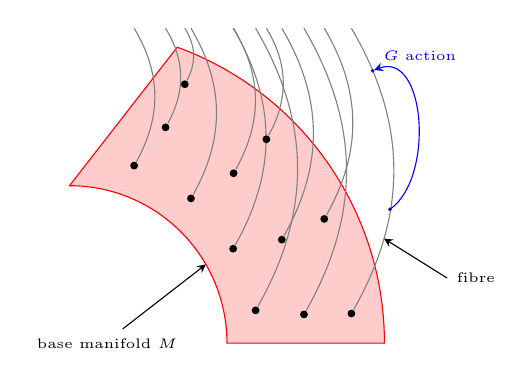
\begin{tikzpicture}[>=stealth]
%\draw[color=red](2,0)--(4,0)node[midway,below]{\textcolor{black}{fibre bundle}}arc(0:70:4)--(90:2)arc(90:0:2)--cycle;
\draw[color=red](2,0)--(4,0)arc(0:70:4)--(90:2)arc(90:0:2)--cycle;
\fill[fill = red, opacity = .2] (2,0)--(4,0)arc(0:70:4)--(90:2)arc(90:0:2)--cycle;

\draw[->] (15:0.7)node[below,xshift=-2mm]{base manifold $M$}--(30:2);

\begin{scope}[bend right]
\foreach \i[count=\x] in {10,30,50,70}
{\node(a\x)[circle,fill,inner sep=1pt]at (\i:2.4){};
\draw[color= gray](a\x)to(a\x|-0,4);}

\foreach \i[count=\x] in {7,26,46,66}
{\node(b\x)[circle,fill,inner sep=1pt]at (\i:3){};
\draw[color= gray](b\x)to(b\x|-0,4);}

\foreach \i[count=\x] in {6,26,46,66}
{\node(c\x)[circle,fill,inner sep=1pt]at (\i:3.6){};
\draw[color= gray](c\x)to(c\x|-0,4);}

\path(c1)to coordinate[near start](d)(c1|-0,4);
\end{scope}
\draw[<-](d)--+(0.8,-0.5)node[right]{fibre};
\draw[->, color=blue](4.07,1.7) to [out=35, in= 20] +(-.2,1.77)node[above right]{$G$ action};
\node(e)[circle, fill, color=blue, inner sep=.5pt] at (4.07,1.7){};
\node(f)[circle, fill, color=blue, inner sep=.5pt] at (3.85,3.46){};

\end{tikzpicture}
\end{document}
